% Description: This file contains the content of the chapter 3 of the dissertation. It is based on an article that me and Grant wrote.

%------------------------------------------------
\chapter{On using Residual H1* for voice quality research} \label{ch:residual_h1}
%------------------------------------------------
%------------------------------------------------
\section{Introduction} \label{sec:Intro}
%------------------------------------------------

Languages use voice quality distinctions to convey phonemic distinctions \citep{garellekPhoneticsVoice2019} and to convey paralinguistic information by ``indexing the biological, psychological, and social characteristics of the speaker" \citep{laverVoiceQualityIndexical1968,podesvaStanceWindowLanguageRace2016}. Voice quality contrasts have been studied extensively by examining their correlates in the acoustic signal \citep[e.g.,][]{espositoCrosslinguisticPatternsPhonation2020}, resulting in a large and complex literature on acoustic correlates of phonation differences \citep[see][]{garellekPhoneticsVoice2019}. 

One measure that Fischer-Jorgensen established, the fundamental's relative strengthive amplitudes of the first harmonic and second harmonic. As established by Fischer-Jorgensen, the relative strength of the fundamental is a correlated measure of breathy voice in contrast with modal voice \citet{fischer-jorgensenPhoneticAnalysisBreathy1968}. In order to normalize the amplitude of the fundamental and counteract some of the effects of high-pass filtering and differences in sound pressure in the signal, she proposed that you could subtract the amplitude of a higher harmonic, in this case, the second harmonic (H2), from the amplitude of the fundamental (H1). Since its introduction, H1*$-$H2* has been used in many studies to measure not only breathy voice but other voice quality contrasts as well \citep{garellekPhoneticsVoice2019,chaiH1H2AcousticMeasure2022}.

Despite the large amount of evidence in support of H1*$-$H2*, it is not without its problems. At the fundamental level, it is not clear that H1*$-$H2* adequately measures the strength of the fundamental. \citet{sundbergObjectiveCharacterizationPhonation2022} found that H1 and H2 are affected differently by subglottal pressure, compromising some of the original reasoning behind the use of H1*$-$H2* from \citet{fischer-jorgensenPhoneticAnalysisBreathy1968}. Similarly, in a comprehensive overview of the main concerns with H1*$-$H2* as a phonation type measure, \citet{chaiH1H2AcousticMeasure2022} found that in addition to the issues mentioned above, errors in measuring H1*$-$H2* are uncomfortably high. This is mainly due to the need to precisely measure two different harmonic amplitudes; when there are errors in calculating H1, this, in turn, leads to errors in calculating H2 \citep{arrasIntroductionErrorPropagation1998}. An example of this type of error propagation is that errors in measuring the fundamental frequency, which is especially common with non-modal phonation, are introduced into measuring harmonics because they are based on the fundamental. Despite algorithms correcting for vowel height, a common error that occurs is when a high fundamental frequency co-occurs with a low first formant \citep{chaiH1H2AcousticMeasure2022}. This situation causes errors in tracking the fundamental frequency and the first formant. A final issue that can occur when measuring the harmonics is in contexts where the vowel is nasalized. \citet{simpsonFirstSecondHarmonics2012} shows that in these nasalized contexts, the first nasal pole (P0) can increase the amplitude of H2 and, when the fundamental frequency is high, H1 increases instead.

This collection of errors leads \citet{chaiH1H2AcousticMeasure2022} to propose a new measure, residual H1*. This measure is calculated by first regressing H1 on energy and then subtracting the product of energy and the energy factor from H1. Chai and Garellek argue that this measure better reflects the initial purpose of using H1*$-$H2*. Furthermore, they find that residual H1*: (i) provides better differentiation between phonation types in !Xóõ; (ii) was more robust for measuring creak in Mandarin with respect to different utterance positions; and (iii) has a stronger relationship to the open quotient than H1*H2* based on a comparison using electroglottogram data.

The contributions \citet{chaiH1H2AcousticMeasure2022} make are very intriguing and have the potential to alter how spectral analyses of voice quality are performed. However, they are not convincing on their own. If residual H1* is to be widely adopted in linguistics, speech pathology, and other speech sciences, then it requires considerable evidence of its effectiveness in acoustic studies. This paper offers additional evidence for residual H1*'s effectiveness. 

Given the promising nature of this measure, we tested residual H1* with data from Santiago Laxopa Zapotec. Although \citet{chaiH1H2AcousticMeasure2022} evaluated residual H1* for !Xóõ and Mandarin, both of which contain tone and voice quality, they do not factor tone into their analysis.\footnote{!Xóõ is most like Zapotec in that it has three phonologized phonation categories. It also has tone, which to our understanding is not restricted by phonation and which is not analyzed in \citet{chaiH1H2AcousticMeasure2022}. The Mandarin case is less relevant as its phonation is prosodic and tonally linked.} This is where testing the effectiveness of residual H1* in Zapotec languages is beneficial. Zapotec languages are often described as laryngeally complex \citep{silvermanLaryngealComplexityOtomanguean1997,ariza-garciaPhonationTypesTones2018}. Laryngeal complexity is defined as a language that allows contrastive tone and contrastive voice quality that are unrestricted in their interactions. This laryngeal complexity between tone and phonation types presents a unique challenge for acoustic analysis and testing of the residual H1* measure. 

Other Zapotec languages have also been studied for voice quality research. For example, \citet{espositoVariationContrastivePhonation2010} found that in Santa Ana del Valle Zapotec there was a biological sex difference in which acoustic measures best capture the voice quality contrasts similar to observations from \citet{klattAnalysisSynthesisPerception1990}. \citet{arellanesarellanesDosGradosLaringizacion2010} found that the realization of laryngealization in a variety of San Pablo Güilá Zapotec is highly variable and depends on the position of laryngealization in the phrase. This was also found to be the case in Betaza Zapotec \citep{crowhurstInfluenceVowelLaryngealisation2016}. \citet{barzilaiContextdependentPhoneticEnhancement2021} found that tone and phrasal position also played a role in how voice quality is realized in San Pablo Macuiltianguis Zapotec. These studies show that Zapotec languages have much to contribute to our understanding of voice quality. 

We find that residual H1* can adequately capture differences in voice quality and is a more robust measure of voice quality than H1*$-$H2*, adding credence to the use of this measure instead of H1*$-$H2* in voice quality research. The remainder of this paper is organized as follows. Section~\ref{sec:SLZ} provides a brief overview of the Santiago Laxopa Zapotec language. Section~\ref{sec:Methods} describes the methods used in the data collection, data processing, and statistical modeling used in this study. Section~\ref{sec:Results} presents the results of the study. Section~\ref{sec:Conclusion} concludes the paper.

%----------------------------------------------------------------------------------------
\section{Santiago Laxopa Zapotec} \label{sec:SLZ}
%----------------------------------------------------------------------------------------
Santiago Laxopa Zapotec is a Northern Zapotec language of the Oto-Manguean language family \citep{adlerAcousticsPhonationTypes2016,adlerDerivationVerbInitiality2018,foleyForbiddenCliticClusters2018,foleyExtendingPersonCaseConstraint2022,sichelPronounsAttractionSierra2020,
sichelFeaturalLifeNominals2020,brinkerhoffDownstepSantiagoLaxopa2021,brinkerhoffTonalPatternsTheir2022}. It is spoken by 981 people in the municipality of Santiago Laxopa, Ixtlán, Oaxaca, Mexico and a small number of other speakers from the diaspora in Mexico and the United States. 

Santiago Laxopa Zapotec exhibits a four-vowel inventory (that is, /i/, /e/, /a/, and /u/), which is further distinguished by a four-way contrast in voice quality. This variety is unique because it is a Northern Zapotec that has developed a breathy voice (/V̤/) in addition to the two types of laryngealization that characterize the rest of the Zapotec languages, namely checked and articulated. Checked vowels are defined as a modal vowel that ends with a period of creaky voice or a glottal closure (/VV̰/ or /Vˀ/ ). Rearticulated vowels are also defined as a modal vowel that also has a period of creakiness or glottal closure but aligned to the middle of a vowel (/VV̰V/ or /VˀV/). This makes an otherwise modal vowel appear as if it is interrupted by this laryngealization.\footnote{This is different from how rearticulated vowels are defined in other languages, where they are a modal vowel followed by an ``echo vowel" which may or may not have a glottal closure intervening between the modal and ``echo" vowel \citep[see][]{bairdPhoneticPhonologicalRealizations2011}. A fuller description of how these vowels are realized in one variety of Zapotec and the terms used are found in \citet{avelinoAcousticElectroglottographicAnalyses2010}.} This difference in laryngeal timing is one of the key differences between these phonations (see \cite{ariza-garciaPhonationTypesTones2018} for a detailed typological study of voice quality distinctions in Zapotec languages).

Santiago Laxopa Zapotec is also tonal with three level tones (H, M, and L) and two contours (MH and HL) appearing in nominals \citep{brinkerhoffTonalPatternsTheir2022}.\footnote{The tonal system of Santiago Laxopa Zapotec for verbs and other lexical categories is still being evaluated.} The language has a complex interaction between tone and phonation types. Every tone can appear with every phonation type, with two exceptions being that breathy voice cannot appear with the high tone and checked voice cannot appear with the rising contour tone. It is unclear whether these are accidental gaps or have a phonetic underpinning.

These interactions between voice quality and tone present a rich environment for testing the reliability of voice quality measures in laryngeally complex languages.

\section{Methods} \label{sec:Methods}
\subsection{Elicitation} \label{sec:Elicitation}

Ten native speakers of SLZ (five female; five male) participated in a wordlist elicitation. Elicitation was performed in the pueblo of Santiago Laxopa, Ixtlán, Oaxaca, Mexico during the summer of 2022 using the built-in microphone of a Zoom H4n handheld recorder (16-bit, 44.5 kHz). 

The wordlist consisted of 72 items repeated three times in isolation and the carrier sentence \textit{Shnia' X chonhe lhas} [ʃnːiaˀ X tʃone ɾas] ``I say X three times''. This sentence was chosen to minimize any effect of the phrasal position \citep[see][for a study about phrasal effects on voice quality in Zapotec]{crowhurstInfluenceVowelLaryngealisation2016}. Additionally, there are no co-articulatory effects on voice quality found with this frame and the items in the wordlist.  Between these 72 words, there were 11 words with breathy voice, 9 with rearticulated voice, 10 with checked voice, and 42 with modal. Thirteen of the 72 words were disyllabic and eight of the thirteen contained the same voice quality in each syllable. Of those 13 disyllabic word, only five contained different voice qualities in each of the syllables. This resulted in 85 different syllables.\footnote{There is ongoing debate about the status of strong syllables in Zapotec. The majority of evidence for the presence of stress comes from non-Northern Zapotec varieties \citep[e.g.,][]{chavez-peonPhoneticCuesStress2008,mockPitchAccentStress1988}. At this time, evidence for stress in Northern Zapotec remains to be seen.} 

The token selection for the wordlist was done in consultation with a native speaker. Similarly to \citet{barzilaiContextdependentPhoneticEnhancement2021}, we did not balance the tones with the different voice qualities. The frequency in which certain tones co-occur with certain voice qualities is uneven in the language, making it difficult to control for. The distribution of tones and voice quality across the 85 syllables used in this study are presented in Table~\ref{tab:distribution}. This imbalance was taken into account by including Tone as a fixed effect in our statistical models in Section~\ref{sec:StatisticalModeling}.

\begin{table}[!h]
  \centering
  \caption{Distribution of tone and voice quality in the wordlist}
  \label{tab:distribution}
    \begin{tabular}{llllll}
    \lsptoprule
    & High & Mid & Low & Rising & Falling\\
    \hline
    Modal & 14 & 9 & 15 & 2 & 10 \\
    Breathy & $-$ & $-$ & 11 & $-$ & 2 \\
    Checked & 1 & $-$ & 9 & $-$ & \\
    Rearticulated & 1 & $-$ & 4 & $-$ & 4 \\
    \lspbottomrule
    \end{tabular}
\end{table}


%----------------------------------------------------------------------------------------
\subsection{Data Processing} \label{sec:DataProcessing}
%----------------------------------------------------------------------------------------

Each vowel of the target words in the carrier sentence condition was labeled following \citet{garellekAcousticDiscriminabilityComplex2020} for where the vowel began and ended. Each vowel in the word list was annotated for speaker, word, vowel, tone, voice quality, and utterance number. This labeling was conducted for each vowel in the target word from the elicitation list of the carrier sentences.

These vowels were then extracted and fed into VoiceSauce for acoustic measurement \citep{shueVoiceSauceProgramVoice2011}. The formants were measured using Snack \citep{sjolanderSnackSoundToolkit2004}, while the fundamental frequency (\textit{f0}) was measured using the STRAIGHT algorithm \citep{kawaharaInstantaneousfrequencybasedPitchExtraction1998}. Spectral slope measures were corrected for formants and bandwidths \citep{hansonGlottalCharacteristicsFemale1997,iseliAgeSexVowel2007}. Each vowel was measured with ten equal time intervals, resulting in 22890 data points in total.

The data were cleaned of outliers following the same steps as taken by \citet{chaiH1H2AcousticMeasure2022} in their study. The H1*, H1*–H2*, and \textit{f0} values were z-scored by speaker to reduce the variation between the speakers and provide a way to directly compare the different measures on the same scale. Data points with an absolute z-score value greater than 3 were considered outliers and excluded from the analyses. Within each vowel category, we calculated the Mahalanobis distance in the F1-F2 panel. Each data point with a Mahalanobis distance greater than 6 was considered an outlier and excluded from the analysis. Using the Mahalanobis distance allows us to compare the data points to the mean of the F1-F2 panel for each vowel category. The larger the Mahalanobis distance is the more deviant the data point is from the mean which in turn means that the data point was improperly tracked. This is comparable to what was done in \citet{seyfarthPlosiveVoicingAcoustics2018,chaiCheckedSyllablesChecked2022,garellekPhoneticsWhiteHmong2023}.

Time points whose \textit{f}0, F1, or F2 values were outliers were also excluded from H1* and H1*$-$H2* analyzes because H1* and H1*$-$H2* are calculated based on \textit{f0}, F1, and F2. Energy was excluded if it had a zero value and then logarithmically transformed to normalize its right-skewed distribution. Afterward, the resulting logarithmically transformed data was z-scored, and any data point with a z-score greater than 3 was excluded. This outlier removal resulted in 1918 datapoints being removed. 

After removing the outliers, we calculated residual H1* for the remaining data points following \citet{chaiH1H2AcousticMeasure2022}. First, a linear mixed effects model was generated with the z-scored H1* as the response variable and the z-scored energy as the fixed effect. The uncorrelated interaction of the z-scored energy by speaker was treated as random. The energy factor resulting from this linear mixed-effects model was extracted. Finally, the z-scored H1* had the product of the z-scored energy and the energy factor subtracted from it, giving us the residual H1* measure.

The measures were then orthogonally coded according to their position in the vowel (first, middle, and third) and for tone (H, M, L, R, F) for statistical modeling.  

%----------------------------------------------------------------------------------------
\subsection{Statistical modeling} \label{sec:StatisticalModeling}
%----------------------------------------------------------------------------------------

Two linear mixed-effects regression models were fitted, one for the normalized H1*$-$H2* and residual H1*. Each model had the tone and the interaction between voice quality and position in the vowel as fixed effects. Vowel and interaction between the speaker, the word, and the repetition were treated as random intercepts.\footnote{ $Measure \sim  Phonation*Position + Tone + (1|Speaker:Word:Repetition) + (1|Vowel)$}

The tone and the interaction between voice quality and position in the vowel were selected as fixed effects for several reasons. The first is that five unique tones appeared in the data and it is well established that tone interacts with voice quality in different ways (see \cite{espositoCrosslinguisticPatternsPhonation2020} and \cite{garellekPhoneticsVoice2019} for discussion). By treating tone as a fixed effect in our model, we can account for these interactions. The interaction between voice quality and position in the vowel as a fixed effect was included to account for the temporal differences between the two different laryngealizations, checked and rearticulated vowels. Checked vowels in Zapotec languages have a glottal occlusion or a short period of creaky voice located at the right edge of the vowel. This is in contrast to rearticulated vowels, where there is a glottal occlusion or creaky voice in the middle of the vowel. Because this difference between checked and rearticulated vowels is temporal in nature, we can account for this difference through the interaction of voice quality and position in the vowel.\footnote{Tone and voice quality are closely linked. By including only the positional interaction with voice quality, we can avoid collinear interactions that appear when we try to include tone in the interaction.}

The interaction between speaker, word, and repetition was treated as a random intercept because this allows us to consider that each speaker said each word on the elicitation list three times. This intercept accounts for not only the intra-speaker variability, but also the inter-speaker variability during each time the word was uttered. Treating a vowel as a random intercept allows us to capture the fact that each voice quality occurred with different vowels during elicitation.

Additional statistical modeling was performed with two generalized additive mixed models (GAMM) using the \texttt{mgcv} package in R \citep{woodGeneralizedAdditiveModels2017}. The GAMMs were fitted to account for any non-linear effects that may be present in the data. In each case the response variable was the same as in the linear mixed-effects models with voice quality as a fixed effect. Splines where used to model the non-linear effects of position and position by phonation. Speaker and word were treated as random intercepts.

%---------------------------------------------------------------------
\section{Results} \label{sec:Results}
%---------------------------------------------------------------------

In interpreting the results, there are certain expectations about how these measures should capture the voice quality contrasts. As discussed in \citet{garellekPhoneticsVoice2019}, it is expected that breathy vowels should have a higher spectral slope than modal vowels across the two measures in keeping with observations about breathy vowels in other languages. Because both checked and rearticulated vowels make use of creaky voice, they should have a lower spectral slope than modal vowels. Additionally, because there is a temporal distinction between checked and rearticulated with where the creakiness appears, this should also be captured in the two measures. 

%---------------------------------------------------------------------
\subsection{\texorpdfstring{H1*$-$H2*}{H1*-H2*}} \label{sec:H1H2}
%---------------------------------------------------------------------

Figure~\ref{fig:FIG1} shows the mean H1*$-$H2* values for each voice quality at each of the ten vowel intervals. We see that the breathy, checked, and rearticulated values are lower than the modal values at each of the first nine intervals. In the final intervals, breathy and rearticulated are essentially equal to the modal value. In contrast, checked's value remains lower than the modal's value throughout the entire vowel. This measure does not match the expectations discussed above.

\begin{figure}[htbp]
  \centering
  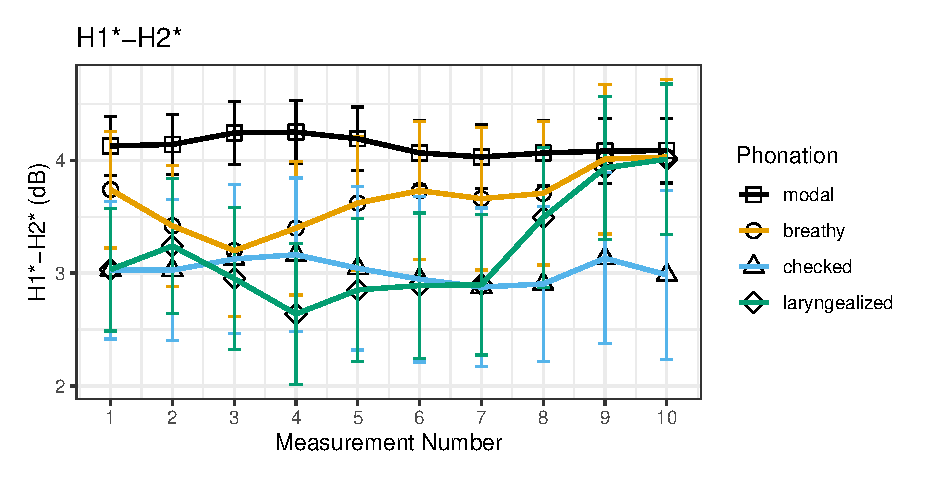
\includegraphics[width = 0.75\textwidth]{images/Figure1.eps}
  \caption{\label{fig:FIG1}{H1*$-$H2* across the duration of the vowel. Points represent the mean of each measure across the ten intervals. The error bars around each point represent a 95\% confidence interval. A line was plotted over each to show how the acoustic measure functions across the ten intervals.}}
\end{figure}

%----------------------------------------------------------------------------------------
\subsection{Residual H1*} \label{sec:ResidH1}
%----------------------------------------------------------------------------------------

Figure~\ref{fig:FIG2} shows the mean residual H1* values for each voice quality at each of the ten vowel intervals. In contrast to Figure~\ref{fig:FIG1}, we see that breathy has a higher residual H1* measure than modal throughout the duration of the vowel, which is consistent with other observations for breathy voice \citep{fischer-jorgensenPhoneticAnalysisBreathy1968}. Checked and rearticulated both have lower values than the modal at each of the 10 intervals. In addition, it shows that the checked voice has a lower residual H1 * value than the rearticulated voice at intervals 8 through 10. The rearticulated voice has a lower residual H1 * value than the checked voice at intervals 1 through 7, showing the temporal distinction between these two voice qualities. This measure complies with the expectations discussed above. 

\begin{figure}[htbp]
  \centering
  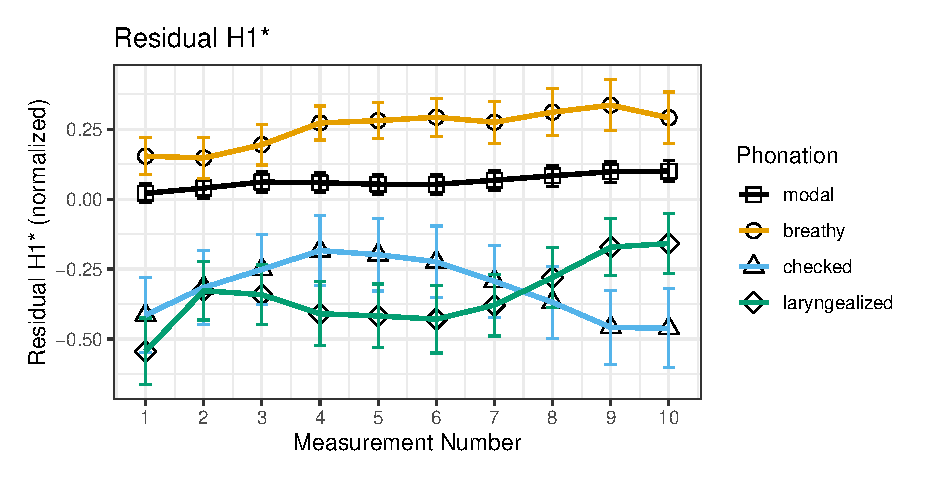
\includegraphics[width = 0.75\textwidth]{images/Figure2.eps}
  \caption{\label{fig:FIG2}{Residual H1* across the duration of the vowel. Points represent the mean of each measure across the ten intervals. The error bars around each point represent a 95\% confidence interval. A line was plotted over each to show how the acoustic measure functions across the ten intervals.}}
\end{figure}


%----------------------------------------------------------------------------------------
\subsection{Model Comparison} \label{sec:Comparison}
%----------------------------------------------------------------------------------------

To assess the robustness of the models, we compared the residual H1* linear mixed-effects model to the H1*$-$H2* linear mixed-effects model. This was done using two methods: direct comparison of the outputs of the two models in the same way as \citet{chaiH1H2AcousticMeasure2022} and the Akaike Information Criterion (AIC). 

Table~\ref{tab:CGComparison} compares the linear mixed effects models for H1*$-$H2* and residual H1*. In comparing these models, we find that the residual H1* model performed better than the H1*$-$H2* model in distinguishing voice quality contrasts in Santiago Laxopa Zapotec. This is supported by the larger absolute value of the coefficient estimate, the lower standard error, and the higher t-value of the residual H1* to distinguish breathy, checked, and rearticulated vowels from modal vowels.

\begin{table}[!h]
  \centering
  \caption{Model comparison between H1*$–$H2* and Residual H1* in distinguishing Santiago Laxopa Zapotec voice quality.}
  \label{tab:CGComparison}
    \begin{tabular}{lllllll}
      \lsptoprule
    Voice Quality Contrast & Model & \textit{$\beta$ } & Std. Error & \textit{t}-value & \textit{p}-value  &     \\
    \hline
      Breathy vs Modal &  H1*$-$H2* & 0.04631 & 0.03806  & 1.21680 & 0.22372 & \\
      & Res. H1* & 0.23625 & 0.02866 & 8.24177   & \textless 0.001   & *** \\
      Checked vs Modal & H1*$-$H2* & -0.11880 & 0.03476 & -3.41793  & \textless 0.001 & *** \\
      & Res. H1* & -0.40099 & 0.02621 & -15.30098 & \textless 0.001 & *** \\
      Rearticulated vs Modal & H1*-H2 & -0.09175 & 0.04588 & -1.99968 & 0.04560 & *  \\
     & Res. H1* & -0.44162 & 0.03450 & -12.80027 & \textless 0.001 & *** \\
     \lspbottomrule
    \end{tabular}
\end{table}

Table~\ref{tab:Comparison} shows the results of the AIC comparison between the H1*$-$H2* and residual H1* models. The residual H1* model had a lower AIC than the H1*$-$H2* model, indicating that the residual H1* model is a better fit for the data than the H1*$-$H2* model. Although AIC comparison is usually performed on nested models, it is still a useful tool for comparing non-nested models \citep{burnhamMultimodelInferenceUnderstanding2004,burnhamAICModelSelection2011,burnhamModelSelectionMultimodel2004}.

\begin{table}[!h]
  \centering
  \caption{AIC for the H1*$-$H2* and residual H1* models.}
  \label{tab:Comparison}
  % \begin{ruledtabular}
  \begin{tabular}{lll}
    \lsptoprule
    Model  & AIC & $\Delta$ AIC\\
    \hline
    H1*$-$H2* model & 43443.33 & 11182.76 \\
    Residual H1* model & 32260.57 & 0 \\
    \lspbottomrule
  \end{tabular}
  % \end{ruledtabular}
\end{table}

%---------------------------------------------------------
\subsection{GAMM analysis and model comparisons} \label{sec:GAMM}
%---------------------------------------------------------

The GAMM analysis shows that there are non-linear effects present in the data. This was expected because of the dynamic nature of the voice quality in SLZ. Figures~\ref{fig:GAMM_h1h2} and \ref{fig:GAMM_residh1} show the GAMM smooths and difference plots for H1*$-$H2* and residual H1*, respectively. The difference plots in each figure show the difference between the smooths for each voice quality compared to modal.

Do to the nature of GAMM analyses, it is important to visually inspect the results to see how well the model fits the data. The model that best fits the data is the one that shows the clearest distinction between the different voice qualities.

In Figure~\ref{fig:GAMM_h1h2}, we see that the different voice qualities are very difficult to observe clearly. In the top left panel, the smooth functions of the GAMM analysis are shown. In it we see that modal and breathy voice occupy the same space. However, checked and rearticulated voice are more separated from modal, with both appearing lower in the graph. The difference plot in the top right show that for breathy vs. modal there was no significant difference between the two voice qualities in term of H1*$-$H2*. In the bottom left, the difference plot shows that the differences we observe between checked and modal voice is significant across the entire duration of the vowel. The difference plot in the bottom right shows that there is a significant difference between rearticulated and modal voice in the first two thirds of the vowel, but not in the final third of the vowel.

\begin{figure}[!ht]
  \centering
  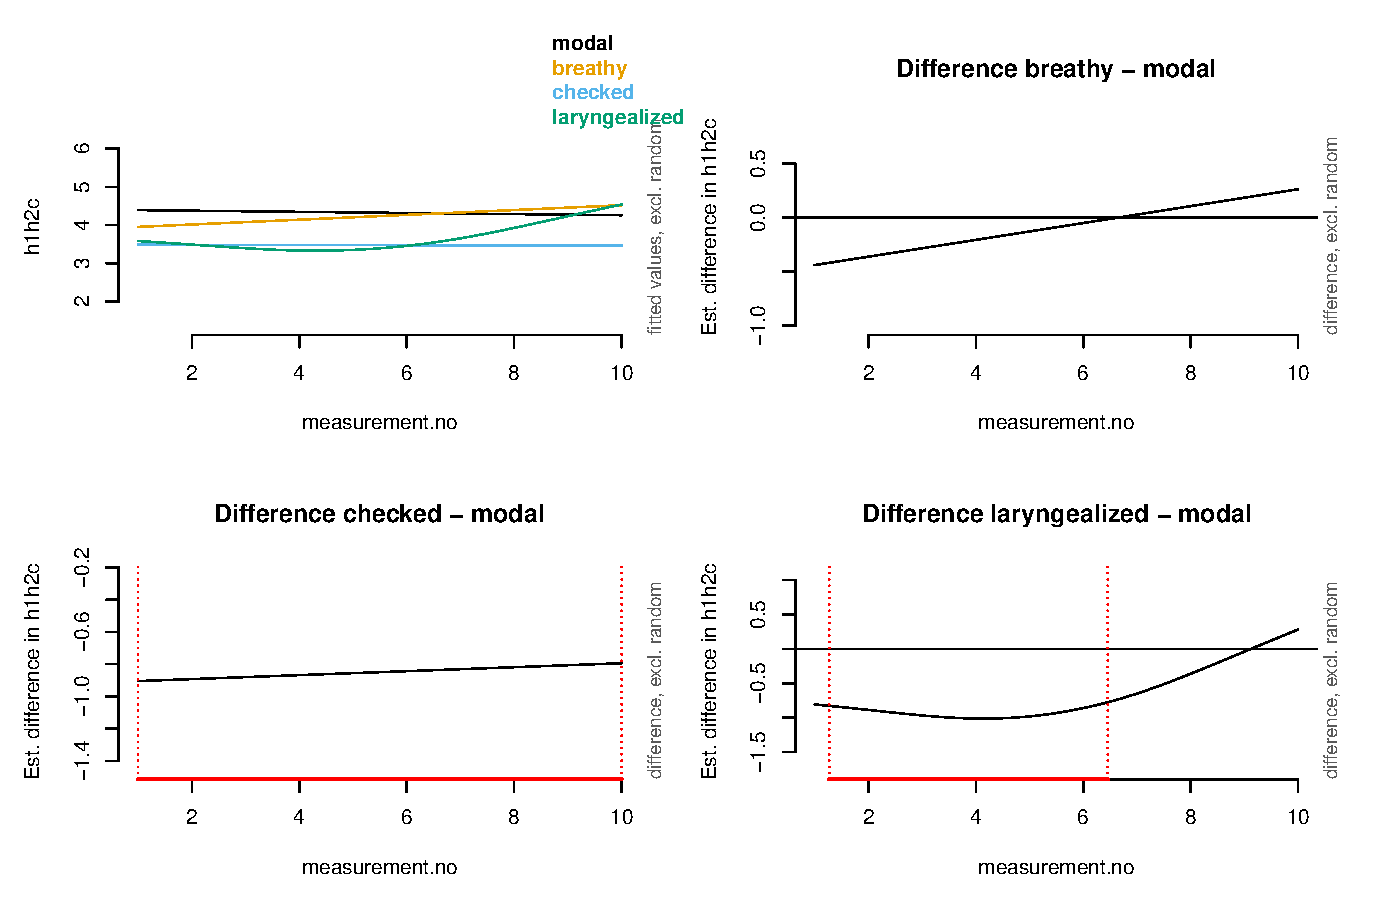
\includegraphics[width = \textwidth]{images/h1h2_gamm.eps}
  \caption{GAMM smooths and difference plots for H1*$-$H2* across the duration of the vowel.}
  \label{fig:GAMM_h1h2}
\end{figure}


The residual H1* GAMM showed a clearer distinction between the different voice qualities than H1*$-$H2*. This is especially clear in the smooth plot where the voice quality distinctions match with the predictions stated above. The difference plot in the top right shows that breathy and modal voice are only significantly different in the final two thirds of the vowel. The bottom left shows that checked and modal voice are significantly different across the entire duration of the vowel. Finally, the bottom right shows that rearticulated and modal voice are significantly different across the entire duration of the vowel.
\begin{figure}[!ht]
  \centering
  \includegraphics[width = \textwidth]{images/residh1_gamm.eps}
  \caption{GAMM smooths and difference plots for residual H1* across the duration of the vowel.}
  \label{fig:GAMM_residh1}
\end{figure}

In comparing the two GAMM analyses, we find that the residual H1* model provides a clearer distinction between the different voice qualities than the H1*$-$H2* model. This is further evidence that residual H1* is a more robust measure of voice quality than H1*$-$H2* in Santiago Laxopa Zapotec. Additionally, the GAMM analysis shows that there appear to be some amount of phasing in the data, which the linear models where unable to capture. This is especially clear in the residual H1* model where the difference plots show that breathy voice is only significantly different from modal in the final two thirds of the vowel. This suggests that breathy voice is aligned with the end of the vowel. This is similar to the predictions made by \citet{silvermanLaryngealComplexityOtomanguean1997,silvermanPhasingRecoverability1997} about the alignment of non-modal phonation in laryngeally complex languages. This will be further discussed in Chapters~\ref{ch:testing_lc} and \ref{ch:modeling_lc}.

\section{Conclusion} \label{sec:Conclusion}

In conclusion, we find that residual H1* is a more robust measure of voice quality than H1*$-$H2* in Santiago Laxopa Zapotec. This is supported by the results of the linear mixed-effects models, which show that residual H1* is better at distinguishing breathy, checked, and rearticulated vowels from modal vowels. This is further supported by the AIC comparison, which shows that the residual H1* model is a better fit for the data than the H1*$-$H2* model. These results lend credence to the claims of \citet{chaiH1H2AcousticMeasure2022} and support using residual H1* instead of H1*$-$H2* in voice quality research, especially in laryngeally complex languages.

However, the results neither suggest nor support the notion that residual H1* should be the sole measure used to determine phonation quality. Instead, we suggest that residual H1* should be included as one of the measures that researchers should consult during their acoustic studies. 